\chapter{Integral quadratic forms.}
\label{chap:integral-quadratic-forms}

{\scshape We have} been studying quadratic forms over a field \(\field\) of characteristic not equal to \(2\) in the first two chapters of this paper (with the exception of \S\S\,\ref{sec:integral-forms-def}--\ref{sec:minimum} of Chapter\,\ref{chap:quadratic-forms}). We shall now turn our attention to quadratic forms over principal ideal domains, and in particular, the ring \(\Integers\) of integers, where the nicer properties of a field do not necessarily hold. We shall mainly do so using the language of lattices, which we shall introduce shortly. This chapter follows closely the exposition in \cite{cassels2008rational}.

As in Chapter\,\ref{chap:quadratic-forms}, by an integral quadratic form we shall mean a form whose associated matrix has only integer entries. Let \(q\) be an integral quadratic form whose associated matrix is \(A = (a_{ij})\). We say that \(q\) is \emph{primitive} if \(\gcd(a_{ij}) = 1\) for all \(i, j\). If at least one of the entries \(a_{ij}\) is odd, then we say that \(q\) is \emph{properly primitive}; otherwise \(q\) is \emph{improperly primitive}. Finally \(q\) is \emph{positive-definite} or \emph{negative-definite} depending as to whether \(q(x) > 0\) or \(q(x) < 0\) for all nonzero \(x\).

\section{Lattice theory.}

\subsection{Definition and properties.}~The notion of lattices provide us with some geometric intuition for the study of integer-valued quadratic forms. A lattice can be thought of as a discrete set of points in \(\Reals^n\) that is ``periodic'' in some sense. One can visualize, for example, the two-dimensional integer lattice is generated by the linearly independent vectors \(\mathbf{e}_1\) and \(\mathbf{e}_2\) as in Fig.\,\ref{fig:lattice}, with the lattice elements following the intuitive geometric operations over a \(2\)-dimensional vector space. We shall now make this notion precise.\label{sec:lattice-def}

\begin{figure}[btp]
    \centering
    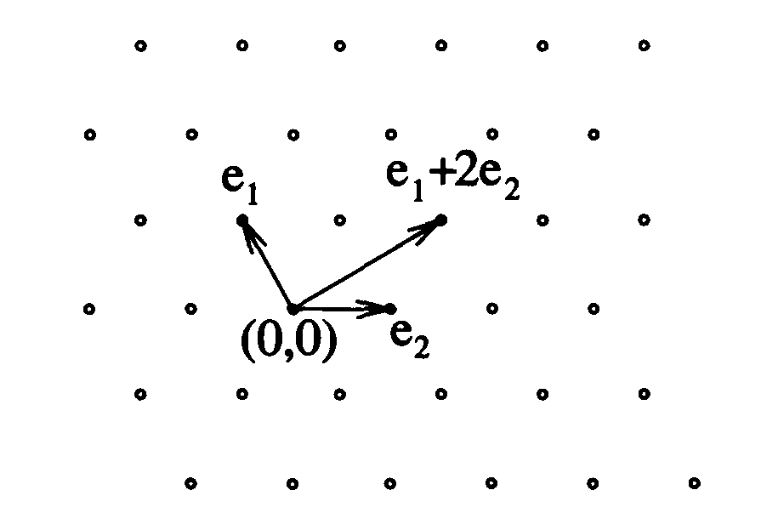
\includegraphics[width=0.6\textwidth]{assets/lattices.png}
    \caption[Visualizing lattices.]{One can visualize a lattice as a discrete set of points in \(\Reals^n\) that is ``periodic'' in some sense. In this figure, the lattice is generated by the linearly independent vectors \(\mathbf{e}_1\) and \(\mathbf{e}_2\).\,\cite{conway1997sensual}}
    \label{fig:lattice}
\end{figure}

Let \(V\) be a \(\field\)-vector space of dimension \(n\) and let \(R\) be a principal ideal domain.\footnote{
    We provide the following definition for completeness: a ring \(R\) is a principal ideal domain if \(R\) is a nonzero commutative ring with no zero divisors (i.e., an integral domain) where every ideal is principal, i.e., generated by a single element. See Chapter III, \S\S\,1--2 of \cite{hungerford2012algebra}. The reader can verify that \(\Integers\) is a principal ideal domain.
} If \(\Basis = \{b_1, \dots, b_n\}\) is a basis of \(V\), then the set
\[
    \Lattice = \{r_1 b_1 + \dots + r_n b_n \}
\]
where each \(r_i\) is an element of \(R\) is called an \emph{\(R\)-lattice} in \(V\) with basis \(\Basis\).

As with \(\field\)-vector spaces, the basis of a lattice is not unique. If \(\Basis' = \{b_1', \dots, b_n'\}\) is another basis of \(V\), then there is an invertible matrix \(M\) with entries in \(R\) such that
\begin{equation}\label{eq:basis-change-lattice-1}
    b_i' = \sum_{j=1}^n m_{ji} b_j;
\end{equation}
similarly, there is a matrix \(M'\) with entries in \(R\) such that
\begin{equation}\label{eq:basis-change-lattice-2}
    b_i  = \sum_{j=1}^n m'_{ji} b'_j.
\end{equation}
Substituting \eqref{eq:basis-change-lattice-1} into \eqref{eq:basis-change-lattice-2}, and using the fact that the elements of \(\Basis\) are linearly independent, we obtain
\[
    \sum m'_{ij}m_{j\ell} =
    \begin{cases}
        \ \ 1 & \text{if } i = \ell,\\
        \ \ 0 & \text{otherwise};
    \end{cases}
\]
whence \((\det M) \cdot (\det M') = 1\) and thus each of \(\det M\) and \(\det M'\) is a unit of \(R\). We can summarize the above result in the following theorem.

\begin{theoremx}
    \label{thm:basis-change-lattice}
    Let \(\Lattice\) be a lattice with basis \(\Basis\) and let \(b'_1, \dots, b'_n\) be elements of \(\Lattice\) given by \(b'_i = \sum_{j=1}^n m_{ji} b_j\), where \(M = (m_{ij})\) is an invertible matrix with entries in \(R\). Then \(\Basis' = \{b'_1, \dots, b'_n\}\) is a basis of \(\Lattice\) if and only if \(\det M\) is a unit of \(R\).
\end{theoremx}

We refer the reader to \cite[pp.\,4--20]{cassels1961geometry} for a more detailed discussion of lattices in the context of the geometry of numbers. We shall now relate our definition of a lattice to the notion of quadratic forms we have thus far developed. Let \((V,B)\) be a quadratic space and let \(q\) be its associated quadratic form. In \S\,\ref{sec:quadratic-maps} we have established that if \(\Basis = \{b_1, \dots, b_n \}\) is a basis of \(V\) and if \(x = (x_1 \dots, x_n)\) is a vector in \(V\), then
\[
    q(x) = \sum B(b_i, b_j) x_i x_j.
\]
Let \(\Lattice\) be an \(R\)-lattice in \(V\) with the same basis \(\Basis\). If we let \(\Basis' = \{b'_1, \dots, b'_n\}\) be another basis of \(\Lattice\) given by \(b'_i = \sum_{j=1}^n m_{ji} b_j\), where \(M = (m_{ij})\) is an invertible matrix with entries in \(R\), then if we define the quadratic form \(q'\) by
\[
    q'(x) = \sum B(b'_i, b'_j) x_i x_j,
\]
we then have
\[
    q'(x) = q\left(\sum_{i=1}^n x_i m_{i1}, \dots, \sum_{i=1}^n x_i m_{in}\right) = q(Mx).
\]
By Theorem\,\ref{thm:basis-change-lattice}, we see that \(q\) and \(q'\) are equivalent over \(R\). Conversely if \(q\) and \(q'\) are equivalent over \(R\), then we can reverse the above argument to see that there is an \(R\)-lattice \(\Lattice\) in \(V\) such that \(q\) and \(q'\) are the quadratic forms associated to \(\Lattice\). We thus have the following theorem.

\begin{theoremx}
    \label{thm:quadratic-form-lattice}
    Let \((V,B)\) be a quadratic space and let \(q\) be its associated quadratic form. Then there is a one-to-one correspondence between the set of \(R\)-lattices in \(V\) and the set of quadratic forms equivalent to \(q\) over \(R\).
\end{theoremx}

We conclude this section with the following theorem and its corollary, the proofs of which the reader can find in \cite[p.\,106--108]{cassels2008rational}.

\begin{theoremx}\label{thm:quadratic-form-lattice-equiv-conditions}
    Let \(R\) be a principal ideal domain contained in some field \(\field\), with \(R \neq \field\). Let \(\Basis = \{b_1, \dots, b_n\}\) be a basis of a the \(R\)-lattice \(\Lattice\) and let \(\beta_1, \dots, \beta_j\) be elements of \(\Lattice\). Then the following statements are equivalent.

    \medskip

    \begin{enumerate}[nosep, label=(\alph*)]
        \item There exist elements \(\beta_{j+1}, \dots, \beta_n\) of \(\Lattice\) such that \(\Basis' = \{\beta_1, \dots, \beta_n\}\) is a basis of \(\Lattice\).
        \item Let \[\beta_{\ell} = \sum_{i=1}^n m_{i\ell} b_i\] for \(1 \leq \ell \leq j\) be the expression of the elements \(\beta_{\ell}\) in terms of the basis \(\Basis\). Then the determinants of the \(j \times j\) minors of the \(j \times n\) matrix \(M = (m_{i\ell})\) are coprime in \(R\).
        \item If \(a = v_1\beta_1 + \dots + v_j\beta_j\) is an element of \(\Lattice\), with \(v_i \in \field\), then \(v_i \in R\) for \(1 \leq i \leq j\).
    \end{enumerate}
\end{theoremx}

\begin{corollary}
    Let \(\beta = v_1b_1 + \dots + v_nb_n\) be an element of \(\Lattice\), with \(\Basis = \{b_1, \dots, b_n\}\) a basis of \(\Lattice\). Then \(\beta\) is a primitive element of \(\Lattice\) if and only if the \(v_i\) are coprime in \(R\).
\end{corollary}

\section{Quadratic forms over \(\IntegersHead_p\) and \(\IntegersHead\).}
\subsection{Integral equivalence.}~In Chapter\,\ref{chap:quadratic-forms} we have defined equivalence of two quadratic forms \(q\) and \(q'\) over a field \(\field\) of characteristic not equal to \(2\) as the existence of an invertible matrix \(T\) such that \(q'(x) = q(Tx)\). We shall now extend this definition to quadratic forms over the ring \(\Integers\) of integers. The reader can verify that the definitions and some of the results in Chapter\,\ref{chap:quadratic-forms}  can be extended to the case when \(\field\) is not a field, but rather a principal ideal domain, as most of the properties we have thus far studied do not necessarily depend on \(\field\) being a field. We thus assume that the results we have thus far studied continue to hold and only call here the reader's attention to the differences. We shall write \(q \sim_{R} q'\) to indicate that the quadratic forms \(q\) and \(q'\) are equivalent over the principal ideal domain \(R\) (or simply \(q \sim q'\) if the ring is clear from context). We shall study \(R\)-equivalence (and more specifically, \(\Integers\)-equivalence) in more detail, following mainly the treatment in \cite{cassels2008rational} and \cite{jones1950arithmetic}.

If a form \(q\) over the principal ideal domain \(R\) represents \(\lambda\), then for any form \(q'\) satisfying \(q \sim_{R} q'\), we know that \(q'\) also represents \(\lambda\). Now if \(q\) has the associated matrix \(M\) and \(q'\) has the associated matrix \(M'\), then we know that \(M' = T^{\transp} M T\) for some invertible matrix \(T\). This brings us to the first significant difference between \(\field\)-equivalence and \(R\)-equivalence. If we let \(\discr q\) and \(\discr q'\) be the respective discriminants of \(q\) and \(q'\), and since \(q \sim_{R} q'\) implies \(M = S^{\transp} M' S\) for some invertible \(R\)-matrix \(S\), then we have
\begin{align*}
    &\discr q = (\det T)^2 \discr q',\text{ and }\\
    &\discr q' = (\det S)^2 \discr q.
\end{align*}
Thus if one of the forms \(q\) and \(q'\) is degenerate, then so is the other. Moreover, limiting our study to nondegenerate forms, we see that
\[
  (\det T)^2 (\det S)^2 = 1,
\]
and hence \(\det T \in R^{\times}\), where \(R^{\times}\) is the group of units of \(R\). If we let \(R = \Integers\), then we see that \(\det T = \pm 1\) since the only units of \(\Integers\) are \(\pm 1\). Thus we have the following result.

\begin{theorem}{\normalfont\cite[p.\,127]{cassels2008rational}}
    Two \(\Integers\)-equivalent quadratic forms have the same discriminant.
\end{theorem}

We say that \(q\) and \(q'\) are properly equivalent over \(\Integers\) if \(q \sim_{\Integers} q'\) and \(\det T = 1\); otherwise we say that they are improperly equivalent. The reader can verify that \(R\)-equivalence is not generally an equivalence relation; nevertheless, proper equivalence over \(\Integers\) is an equivalence relation. Before we continue studying equivalence in \(\Integers\), we shall first review some properties of quadratic forms over the ring \(\Integers_p\) of \(p\)-adic integers.

\subsection{The lattice \(\Integers_p^n\)}~Let \(p\) be a prime number and never the symbol \(\infty\). As in Chapter\,\ref{chap:local-global-principle}, we write \(\Integers_p^n\) we mean the set of \(n\)-tuples \((a_1, \dots, a_m)\) where each \(a_i\) is a \(p\)-adic integer. The reader can verify that \(\Integers_p^n\) is a lattice on \(\Rationals_p^n\). This observation, together with the fact that \(\Integers_p^n\) is an integral domain, leads us to the following special case of Theorem\,\ref{thm:quadratic-form-lattice-equiv-conditions} of \S\,\ref{sec:lattice-def}.\label{sec:the-lattice-zpn}

\begin{theorem}
    {\normalfont\cite[p.\,112]{cassels2008rational}}
    Let \(\beta_1, \dots, \beta_j\) be independent elements of \(\Integers_p^n\). Then the following statements are equivalent.

    \medskip

    \begin{enumerate}[nosep, label=(\alph*)]
        \item There exist elements \(\beta_{j+1}, \dots, \beta_n\) of \(\Integers_p^n\) such that \(\Basis' = \{\beta_1, \dots, \beta_n\}\) is a basis of \(\Integers_p^n\).
        \item The \(n \times j\) matrix \(\beta_1 \beta_2 \dots \beta_j\) contains a \(j \times j\) minor whose determinant is a unit of \(\Integers_p\).
        \item If \(a = v_1\beta_1 + \dots + v_j\beta_j\) is an element of \(\Integers_p^n\), with \(v_i \in \Rationals_p\), then \(v_i \in \Integers_p\) for \(1 \leq i \leq j\).
    \end{enumerate}
\end{theorem}

As in \S\,\ref{sec:lattice-def} we have the following corollary:

\begin{corollary}
    A vector in \(\Integers_p^n\) forms part of a basis of \(\Integers_p^n\) if and only if it is a primitive element of \(\Integers_p^n\).
\end{corollary}

\subsection{Canonical forms in \(\Integers_p\).}~We shall now show that every quadratic form over \(\Rationals_p\) has an integral automorph of determinant \(-1\): this fact will be useful later on in our study of genera. We then restrict our attention to the case \(p \neq 2\)\footnote{Here \(p\) is a prime and never the symbol \(\infty\).} and show the existence of a set \(\mathcal{C}\) of canonical forms over \(\Integers_p\) such that every quadratic form over \(\Rationals_p\) is \(\Integers_p\)-equivalent to a form in \(\mathcal{C}\). An exposition of the case \(p = 2\) can be found in Chapter 8, \S\,4 of \cite{cassels2008rational}.\label{sec:canonical-forms-zp}

Let \(q\) be a nondegenerate form over \(\Rationals_p\). Then for any \(x \in \Integers_p\), \(|q(x)|\) is bounded above, and because (cf. \S\,\ref{sec:quadratic-maps})
\[
    2B(x, y) = q(x+y) - q(x) - q(y),
\]
with \(x\) as before and \(y\) also a \(p\)-adic integer, we have
\[
    \sup_{x, y \in \Integers_p} |2B(x, y)| < \sup_{x \in \Integers_p} |q(x)|.
\]
The suprema on both sides exists since the \(p\)-adic valuation is nonarchimedean. Thus there is a \(p\)-adic integer \(x_0\) such that \(|q(x_0)|\) is maximal, i.e., equal to \(\sup |q(x)|\). Moreover, \(x_0\) must be a primitive element of \(\Integers_p\), for if \(x_0 = py\) for some \(y \in \Integers_p\), then \(q(x_0) = q(py) = p^2 q(y)\). This gives us the following lemma.

\begin{lemmax}\label{lemma:q-primitive}
    A quadratic form \(q\) over \(\Rationals_p\) is \(\Integers_p\)-equivalent to a form \(q'\) with
    \[
        |q'(1, 0, \dots, 0)| = \sup_{x \in \Integers_p^n} |q'(x)|.
    \]
\end{lemmax}

\begin{proof}
    Apply the theorem of \S\,\ref{sec:the-lattice-zpn} to show the existence of a \(p\)-adic integer \(y\) such that \(|q(y)|\) is maximal.
\end{proof}

\begin{lemmax}\label{lemma:tau-y}
    Let \(y\) be a \(p\)-adic number such that \(q(y) \neq 0\) and with \(y\) maximal in \(q\), where \(q\) is a quadratic form over \(\Rationals_p\). Then the map
    \[
       \tau_y : x \mapsto x - \frac{B(x,y)}{f(y)}y
    \]
    is a \(\Integers_p\)-automorphism of \(q\) with determinant \(\ -1\).
\end{lemmax}

\begin{proof}
    The composition \((\tau_y)^2\) is the identity map and thus we need only show that the image of any element of \(\Integers_p^n\) under \(\tau_y\) is also an element of \(\Integers_p^n\). Let \(x \in \Integers_p^n\). Then since \(\sup |2B(x, y)| < \sup |q(x)|\), and by our maximality assumption on \(y\), we have
    \[
        \sup |2B(x, y)| < |q(y)|,
    \]
    and thus \(2B(x, y)/q(y) \in \Integers_p^n\) and the result follows. By routine computation we can show that \(\det \tau_y = -1\).
\end{proof}

We now show some results concerning quadratic forms over \(\Integers_p\) for \(p \neq 2\).

\begin{lemmax}\label{lemma:tau-z}
    If \(z, z' \in \Integers_p^n\) and \(q\) is a quadratic form over \(\Rationals_p\) such that \(q(z) = q(z')\) and \(|q(z)|\) and \(|q(z')|\) are maximal, then there is a \(\Integers_p\)-automorphism \(\sigma\) of \(q\) such that \(\sigma(z) = z'\).
\end{lemmax}

\begin{proof}
    By routine calculation we have
    \[
        |q(z + z') + q(z - z')| = \sup |q(x)|,
    \]
    and thus either of \(|q(z - z')|\) or \(|q(z + z')\) is maximal. In the first case, we can apply Lemma\,\ref{lemma:tau-y} with \(y = z - z'\) and define the automorphism \(\sigma\) as \(\tau_y\). In the second case, put \(y = z + z'\) and define \(\sigma\) as \(\tau_y\tau_{z}\).
\end{proof}

\medskip

Lemma\,\ref{lemma:tau-z} has the following corollary.

\begin{corollary}
    Let \(\sigma\) be a \(\Integers_p\)-automorphism of a quadratic form \(q\) over \(\Rationals_p\). Then \(\sigma\) is the product of \(\Integers_p\)-automorphisms of the form \(\tau_y\) (as defined in Lemma\,\ref{lemma:tau-y}) with integral \(y\).
\end{corollary}

\begin{lemmax}
    Let \(u_1, \dots, u_n\) be \(p\)-adic units. Then the form
    \[
        q(x) = u_1 x_1^2 + \dots + u_n x_n^2
    \]
    is \(\Integers_p\)-equivalent to the form
    \[
        q'(x) = x_1^2 + \dots + x_{n-1}^2 + ux_n^2.
    \]
    where \(u = u_1 \cdots u_{n}\).
\end{lemmax}

\begin{proof}
    Adapt the induction argument in the proof of Theorem\,\ref{thm:quadratic-forms-fq-rank-n} of \S\,\ref{sec:quadratic-forms-fq} on the rank \(n\) of \(q\).
\end{proof}

\begin{theoremx}
    {\normalfont\cite[p.\,115--116]{cassels2008rational}}
    Let \(p\) be an odd prime and let \(r\) be some fixed quadratic non-residue of \(p\). For \(\epsilon \in \{0, 1\}\) and for \(m = 1, 2, \dots\), let \(t(y) = t(\epsilon, m, y)\) be the quadratic form
    \[
        t(\epsilon, m, y) = \begin{cases}
            \ \ y_1^2 + \dots + y_m^2 & \text{if } \epsilon = 0,\\
            \ \ y_1^2 + \dots + y_{m-1}^2 + r y_m^2 & \text{if } \epsilon = 1.
        \end{cases}
    \]
    Then every nondegenerate form \(q\) over \(\Rationals_p\) is \(\Integers_p\)-equivalent to a form of the type
    \begin{equation}\label{eq:canonical-forms}
        q'(x) = \sum_{i=1}^M p^{e_i} t(\epsilon_i, m_i, y^{(i)})
    \end{equation}
    for some \(M\), some \(e_i\) with \(e_1 < e_2 < \dots < e_M\) and some \(\epsilon_i\) and \(m_i\) with \(\sum m_i = n\).\footnote{Here we write \(y^{(1)}\) to avoid ambiguity in indexing the vectors of the form \(y = (y_1, \dots, y_n)\).}
\end{theoremx}

\begin{proof}
    By Lemma\,\ref{lemma:q-primitive}, \(q\) is equivalent to a form \(\sum a_{ij}x_{ij}\) where \(|a_{11}| \geq |a_{ii}|\). Since \(p \neq 2\), we also have \(|a_{11}| \geq |a_{ij}|\) and thus
    \[
        q(x) = a_{11}\left(x_1 + \frac{a_{12}}{a_{11}}x_2 + \dots + \frac{a_{1n}}{a_{11}}x_n\right)^2 + r(x_2, \dots, x_n),
    \]
    for some form \(r\), where each \(a_{ij}/a_{11}\) is a \(p\)-adic integer. Thus \(q\) is \(\Integers_p\)-equivalent to \(a_{11}x_1^2 + h(x)\) and by induction to the diagonal form \(\quadform{a_{11}, \dots, a_{nn}}\) satisfying
    \[
        |a_{11}| \geq |a_{22}| \geq \dots \geq |a_{nn}|.    
    \]
    Combining similar terms, we can write \(\quadform{a_{11}, \dots, a_{nn}}\) as
    \[
        \sum_{i=1}^M p^{e_i} q'_i(y^{(i)}),
    \]
    where \(q'_i\) is a form of the type \(\quadform{u_1, \dots, u_n}\) where the \(u_i\) are \(p\)-adic units. By the previous lemma, each \(q'_i\) is \(\Integers_p\)-equivalent to \(\quadform{1, 1, \dots, u}\) where \(u = u_1 \cdots u_n\). Thus either \(u = v^2\) or \(u = rv^2\) for some other \(p\)-adic unit \(v\), with \(r\) as in the statement of the theorem. This shows that \(q\) is \(\Integers_p\)-equivalent to a form given by \eqref{eq:canonical-forms}.

    It remains to show that \(q\) determines the form given by \eqref{eq:canonical-forms} uniquely. Taking \(p^eq\) instead of \(q\) for a suitable integer \(e\), we can suppose that \(q\) is a primitive form over \(\Integers_p\). We can thus construct \(q'\) as follows: if \(q\) represents the square of a unit then split \(\quadform{1}\), otherwise it represents \(r\) and we can thus split \(\quadform{r}\). By Lemma\,\ref{lemma:tau-y} any two representations of \(\quadform{1}\) or of \(\quadform{r}\) are equivalent unde the group of integral automorphs. The uniqueness of the form given by \eqref{eq:canonical-forms} follows by induction on the rank \(n\) of \(q\).
\end{proof}

\medskip

This theorem has the following useful corollary.

\begin{corollary}
    Suppose that \(q\) and \(q'\) are integral forms such that \(\discr q = \discr q'\) is a \(p\)-adic unit. Then \(q\) and \(q'\) are \(\Integers_p\)-equivalent.
\end{corollary}

We conclude this section by providing the following approximation theorem. See \cite[p.\,126--127]{cassels2008rational} for a proof.

\begin{theoremx}\label{thm:approximation-zp}
    Let \(q\) be a nondegenerate quadratic form over \(\Integers_p\) with discriminant \(\discr q\) and define \(\delta\) by \(|d| = p^{-\delta}\) and \(\zeta\) as \(1\) if \(p = 2\) and \(0\) otherwise. Then if \(r\) is another form with discriminant \(\discr r\) satisfying \(\discr r = u^2\cdot \discr q\) where \(u\) is a \(p\)-adic unit, and
    \[
        r_{ij} \equiv q_{ij} \pmod{p^{\delta + 2\zeta}},  
    \]
    where \(r_{ij}\) and \(q_{ij}\) are the \(ij\)-th entries of the matrices associated with \(r\) and \(q\) respectively, then \(r\) is \(\Integers_p\)-equivalent to \(q\).
\end{theoremx}

\subsection{Reduction, redux.}~We now revisit the reduction theory of integral quadratic forms we have introduced in \S\S\,\ref{sec:integral-forms-def}--\ref{sec:minimum} of Chapter\,\ref{chap:quadratic-forms}. The goal of this section is to prove a finiteness theorem for nondegenerate integral quadratic forms of a given rank. We begin with a couple of lemmas.\label{sec:integral-reduction-redux}

\begin{lemmax}\label{lemma:theta-inequality}
    {\normalfont\cite[p.\,136]{cassels2008rational}}
    For all pairs of integers \(r \geq 1\) and \(s \geq 0\) there is a constant \(\theta := \theta(r, s)\) such that if \(q\) is a quadratic form of rank \(n\) that is \(\Reals\)-equivalent to the form
    \[
        \xi_1^2 + \dots + \xi_r^2 - \xi_{r+1}^2 - \dots - \xi_{r+s}^2,
    \]
    (with \(n = r + s\), cf. \S\,\ref{sec:representation-in-qp-sec}), then there is an integral vector \(a\) such
    \[
        0 < q(a) \leq \theta |\discr q|^{1/n}.
    \]
    Furthermore, \(\theta\) can be taken to be
    \begin{equation}
        \label{eq:theta-inequality}
        \theta^n = 3^s (4/3)^{n(n-1)/2}.
    \end{equation}
\end{lemmax}

\emph{Proof.} The case \(n = 1\) is trivial; we may thus suppose that \(n \geq 2\) and proceed by induction on the rank \(n\) of \(q\). Consider the vector \(a\) satisfying \(q(a) = \min q\) (here we use the assumption that \(q\) is integral); the vector \(a\) is primitive and finding an appropriate quadratic form for \(q\) we may suppose that
\[
    \min q = q(1, 0, \dots, 0).
\]
Thus we have, for some quadratic form \(r\),
\[
    \min q \cdot q(x) =(\min q x_1 + a_{12} x_2 + \dots + a_{1n} x_n)^2 + q'(x_2, \dots, x_n),
\]
where \(a_{ij}\) are the entries of the matrix \(A\) associated to \(q\). We have further that
\[
    \discr q' = (\min q)^{n-2}\discr q.
\]
We now have two cases:

\medskip

\begin{enumerate}[wide, nosep, label=(\roman*)]
    \item If \(r > 1\), then using induction we can apply the lemma to \(q'\) (with \((r-1, s)\) instead of \((r, s)\)) to obtain a vector \(b = (b_2, \dots, b_n)\) such that
    \[
        0 < g(b_2, \dots, b_n) \leq \theta_1\,|(\min q)^{n-2} \discr q|^{1/(n-1)},
    \]
    where \(\theta_1 = \theta(r-1, s)\). Choosing an integer \(b_1\) such that
    \[
        |\min q\cdot b_1 + a_{12} b_2 + \dots + a_{1n} b_n| \leq \frac{1}{2}\min q
    \]
    gives us \(f(b) > 0\), where \(b = (b_1, \dots, b_n)\). By the minimality of \(\min q\), we have, further, that \(f(b) > \min q\). Thus we have
    \[
        \min q \cdot f(b) \leq \frac{1}{4}(\min q)^2 + \theta_1\,|(\min q)^{n-2} \discr q|^{1/(n-1)},
    \]
    whence, eliminating \(f(b)\), we obtain
    \[
        (\min q)^n \leq (4\theta_1/3)^{n-1} |\discr q|,
    \]
    so that we may take \(\theta^n = (4\theta_1/3)^{n-1}\), as desired.

    \item If \(r = 1\), then using induction we can apply the lemma to \(-q'\) (with \((s,0)\) instead of \((r, s)\)) to obtain a vector \(b = (b_1, \dots, b_n)\) such that
    \[
        0 > g(b_2, \dots, b_n) \geq -\theta_2\,|(\min q)^{n-2} \discr q|^{1/(n-1)},
    \]
    where \(\theta_2 = \theta(s, 0)\). Choosing an integer \(b_1\) such that
    \[
        \frac{1}{2}\min q \leq |\min q\cdot b_1 + a_{12} b_2 + \dots + a_{1n} b_n| \leq \min q
    \]
    gives us \(f(b) < \min q\), whence \(f(b) \leq 0\). Arguing as in the first case above we obtain
    \[
        (\min q)^n \leq (4\theta_2)^{n-1} |\discr q|,
    \]
    so that we may take \(\theta^n = (4\theta_2)^{n-1}\), as desired.
\end{enumerate}

Finally, \eqref{eq:theta-inequality} follows from induction on the value of \(\theta^n\) in the two cases above. {\scshape q.e.d.}

\medskip

A corollary to Lemma\,\ref{lemma:theta-inequality} is a generalization of the Hermite bound we have introduced in \S\,\ref{sec:minimum}.\footnote{The results in this section are indeed mainly due to Hermite, as originally published in his letters to Jacobi. \cite{hermite1850extraits}}

\begin{corollary}
    Let \(q\) be a real-valued nondegenerate quadratic form of rank \(n\). Then there is a nonzero integral vector \(a\) such that
    \[
        |q(a)| \leq (4/3)^{n(n-1)/2} |\discr q|^{1/n}.
    \]
\end{corollary}

Lemma\,\ref{lemma:theta-inequality} has the following lemma as another corollary.

\begin{lemmax}
    {\normalfont \cite[p.\,135]{cassels2008rational}}
    Let \(q\) be a nondegenerate integral quadratic form of rank \(n\). Then there exists a nonzero integral vector \(a\) such that for each \(n \geq 1\) there is a constant \(C_n\) such that
    \[
        |q(a)| \leq C_n |\discr q|^{1/n}.
    \]
\end{lemmax}

\begin{theorem}[Finiteness theorem]
    {\normalfont \cite[p.\,129]{cassels2008rational}}
    There are only finitely many \(\Integers\)-equivalence classes of nondegenerate integral quadratic forms of rank \(n\).
\end{theorem}

\begin{proof}
    We can suppose without loss of generality that the vector \(x\) in Lemma\,\ref{lemma:theta-inequality} is primitive: indeed if \(x = \lambda x'\) for some integer \(\lambda\) and an integral vector \(x'\), then \(|f(x')| < |f(x)|\). Let \(t = q(x)\) so that \(t\) belongs to a finite set of nonzero integers depending only on \(n\) and \(\discr q\). Since \(x\) is primitive, \(q\) is \(\Integers\)-equivalent to a form
    \[
        q^*(x) = \sum a_{ij}x_i x_j
    \]
    where \(a_{ij} = t\). By completing the square we then obtain
    \begin{equation}\label{eq:completing-the-square-z}
        tq^*(x) = (tx_1 + a_{12}x_2 + \dots + a_{1n}x_n)^2 + q'(x_2, \dots, x_n),
    \end{equation}
    for some quadratic form \(q'\) of rank \(n-1\). We can then compute the discriminant of \(q'\) to be \(t^{n-2} \discr q\). Thus we can suppose that \(q'\) is equivalent to one of a finite set of forms by induction on the rank \(n\) of \(q\). Keeping \(x_2, \dots, x_n\) fixed we can make the substitution \(x_1 \mapsto x_1 + u_2 x_2 + \dots + u_n x_n\) where the \(u_i\) are integers such that \(|a_{ij}| \leq |t|\) for \(2 \leq j \leq n\). Hence the right-hand side of \eqref{eq:completing-the-square-z} is one of a finite set of forms depending only on \(n\), \(t\) and \(\discr q\). Since the set of integers \(t\) is finite, the result follows.
\end{proof}


\section{Theory of genera.}

\subsection{Basic properties of genera.}~We now introduce the notion of the genus. We say that two nondegenerate quadratic forms \(q\) and \(q'\) are in the same \emph{genus} if they are equivalent in every \(\Integers_v\) for all places \(v\) of \(\Integers\), that is,
\[
    q(x) = q'(M_v x)
\]
where the matrix \(M_v\) has elements in \(\Integers_v\) and \(\det M_v\) is a unit of \(\Integers_v\) for all \(v \in \Places\). In this section we shall prove some basic properties of genera.\label{sec:basic-properties-of-genera}

\begin{theoremx}\label{thm:genus-same-discr}
    {\normalfont \cite[p.\,140]{cassels2008rational}}
    Two forms in the same genus have the same discriminant.
\end{theoremx}

\begin{proof}
    We have, for arbitrary forms \(q\) and \(q'\) belonging to the same genus,
    \[
        \discr q = (\det M_v)^2 \discr q',
    \]
    so that \(\discr q/\discr q'\) is a \(v\)-adic unit for all \(v \in \Places\) and hence must be \(\pm 1\). When \(v = \infty\), we see that \(\discr q\) and \(\discr q'\) have the same sign.
\end{proof}

Theorem\,\ref{thm:genus-same-discr} allows us to speak of the discriminant of a genus, referring, of course, to the discriminant of any form in the genus. From the above theorem and the theorem of \S\,\ref{sec:integral-reduction-redux} we can deduce the following corollary.

\begin{corollary}
    The number of equivalence classes in a genus is finite.
\end{corollary}

The following theorem will be used in \S\,\ref{sec:genus-existence} but involves results in \(p\)-adic analysis which we have not covered in this paper. See \cite[p.\,140]{cassels2008rational} for a proof.

\begin{theoremx}
    \label{thm:genus-topology}
    Let \(P\) be a finite set of primes, excluding the symbol \(\infty\), and let \(q\) be an integral quadratic form with nonzero determinant \(\discr q\). For each \(p \in P\) let \(q_p\) be the \(\Integers_p\)-integral form with discriminant \(\discr q\) that is \(\Integers_p\)-equivalent to \(q\). Then there is a form \(q'\) that is properly equivalent to \(q\) and whose coefficients are arbitrarily close to those of each of the forms \(q_p\) in the \(p\)-adic topology.
\end{theoremx}

\subsection{Existence of genera under local conditions.}~As we have show in Chapter\,\ref{chap:local-global-principle}, the existence of a ``local'' solution in \(\Rationals_p\) does not guarantee the existence of a solution in \(\Rationals\). By the Hasse-Minkowski theorem, however, a solution in \(\Rationals\) exists if and only if solutions exist in \(\Rationals_p\) for all \(p\) including \(p = \infty\). One can see that the Hasse-Minkowski theorem does not generalize to quadratic forms over \(\Integers\) and \(\Integers_p\). If \(q\) represents an integer \(\lambda\) in \(\Integers_p\) for all \(p\), then \(q\) does not necessarily represent \(\lambda\) in \(\Integers\). However, we shall prove in this section that \(\lambda\) must be represented by some form in the genus of \(q\). We begin with the following theorem.\label{sec:genus-existence}

\begin{theoremx}\label{thm:genus-existence}
    {\normalfont \cite[p.\,129, 141--143]{cassels2008rational}}
    Let \(n \geq 1\) and \(\discr \neq 0\) be integers. For each prime \(p \neq \infty\), let \(q_p\) be a quadratic form of rank \(n\) over \(\Integers_p\) with determinant \(\discr\). Suppose that there exists a rational form \(r\) that is \(\Rationals_p\)-equivalent to \(q_p\) for all \(p\). Then there is a form \(q\) that is \(\Integers_p\)-equivalent to \(q_p\) for all \(p\) and \(\Rationals\)-equivalent to \(r\).
\end{theoremx}

If \(n = 1\), then \(q_p(x) = \discr \cdot x_1^2\)\footnote{We write \(\discr \cdot x\) to indicate that \(\discr\) is not being used here as an operator but rather as a scalar.} for all \(p\). Thus we can simply let \(q(x) = \discr \cdot x_1^2\) and the theorem holds. We may therefore suppose that \(n \geq 2\) and proceed by induction on \(n\). The following lemma will be useful:

\begin{lemma}
    Let \(n \geq 2\) and suppose that the theorem holds for \(n - 1\). Let \(\discr\), \(q_p\) and \(r\) be as in the statement of the theorem for \(n\) and let \(\lambda \neq 0\) be the (rational) integer represented by each \(q_p\) over \(\Integers_p\) and by \(r\) over \(\Reals = \Integers_{\infty}\). Then there is a form \(q\) satisfying the conditions of the theorem and representing \(\lambda\) over \(\Integers\).
\end{lemma}

\emph{Proof of Theorem} \ref{thm:genus-existence} \emph{and the lemma.} We begin by proving the lemma. Replacing \(q_p\) for each \(p\) by a \(\Integers_p\)-equivalent form as needed, we may assume without loss of generality that \(q_p(1, 0, \dots, 0) = \lambda\) for all \(p\).

By the Hasse-Minkowski theorem, the form \(r\) represents \(\lambda\) over \(\Rationals\) and so, replacing \(r\) by a \(\Rationals\)-equivalent form as needed, we may suppose that \(r(1 ,0, \dots) = a\). By completing the square we then have
\begin{equation}\label{eq:lambda-qp}
    \lambda q_p(x) = (\lambda x_1 + b_{2p}x_2 + \dots + b_{np}x_n)^2 + q'(x_2, \dots, x_n),  
\end{equation}
for some \(b_{2p}, \dots, b_{np} \in \Integers_p\), where \(q'\) is a quadratic form of rank \(n-1\) over \(\Integers_p\) with determinant \(\discr q' = \lambda^{n-2} \discr q\). Similarly,
\begin{equation}\label{eq:lambda-r}
    \lambda r(x) = (\lambda x_1 + c_2x_2 + \dots + c_nx_n)^2 + r'(x_2, \dots, x_n),
\end{equation}
for some \(c_2, \dots, c_n \in \Rationals\) and some rational quadratic form \(r'\) of rank \(n-1\).

Since \(q_p\) and \(r\) are \(\Rationals_p\)-equivalent, it follows that, by \eqref{eq:lambda-qp} and \eqref{eq:lambda-r}, Witt's lemma implies that \(q'\) and \(r'\) are \(\Rationals_p\)-equivalent. thus \(q'_p\) together with \(\discr q'\) and \(r'\) satisfy the inductive hypothesis of the lemma. It therefore follows that there is an integral form \(q'\) of discriminant \(\discr q'\) that is \(\Integers_p\)-equivalent to \(q'_p\) for all \(p\) and \(\Rationals\)-equivalent to \(r'\).

We can replace \(q'\) with an equivalent form and suppose, by Theorem\,\ref{thm:genus-topology} of \S\,\ref{sec:basic-properties-of-genera} that \(q'\) is arbitrarily close in the \(p\)-adic sense to \(q'_p\) for all \(p\) dividing \(2 \lambda\discr\). Moreover, by the Chinese Remainder Theorem, we can find integers  \(b_2, \dots, b_n\) that are arbitrarily close \(p\)-adically to \(b_{2p}, \dots, b_{np}\) for all \(p \mid 2 \lambda \discr\). Let
\begin{equation}\label{eq:q-definition-lemma}
    q(x) = \lambda^{-1}(\lambda x_1 + b_2x_2 + \dots + b_nx_n)^2 + \lambda^{-1}q'(x_2, \dots, x_n).
\end{equation}
Then \(q\) has discriminant \(\discr q\) and is arbitrarily close to \(q_p\) for all \(p | 2\lambda\discr\). The form \(q\) can also be seen to have rational coeeficients as it was obtained by dividing an integral form by \(\lambda\). However, the coefficients of \(q\) may be made integers by choosing \(q\) sufficiently close to \(q_p\) for the \(p\) dividing \(\lambda\), which we shall suppose.

Since \(q\) is arbitrarily close to \(q_p\) in the \(p\)-adic sense for all \(p \mid 2 \lambda \discr\), we can ensure that \(q\) and \(q_p\) are \(\Integers_p\)-equivalent by Theorem\,\ref{thm:approximation-zp} of \S\,\ref{sec:canonical-forms-zp} for those \(p\). Thus \(q\) and \(q_p\) are \(\Integers_p\)-equivalent for all \(p\). Since \(q'\) and \(r'\) are \(\Rationals\)-equivalent, \(q\) and \(r\) are \(\Rationals\)-equivalent. By our definition of \(q\) in \eqref{eq:q-definition-lemma}, \(q(1,0,\dots, 0) = \lambda\), and thus \(\lambda\) is primitively represented by \(q\). This proves the lemma.

\medskip

To prove the theorem, we suppose that the theorem holds for \(n - 1\). By the lemma, it suffices to show that an integer \(\lambda\) exists satisfying the conditions of the lemma. Let \(\mu\) be any nonzero integer represented by \(r\) over \(\Rationals\) and let \(P\) be the set of primes that divide \(2\mu\discr\). Since there is only one \(\Integers_p\)-equivalence class for each \(p \in P\), \(\mu\) is represented primitively by \(q_p\) over \(\Integers_p\) for such \(p\)'s. For \(p \notin P\), \(q_p\) represents \(\mu\) over \(\Rationals_p\) because \(q_p\) and \(r\) are \(\Rationals_p\)-equivalent by the hypothesis. If \(\mu = q(\mu_p)\), with \(\mu_p \in \Rationals_p^n\), we may choose \(m_p \in \Integers\) such that \(p^{m_p}\mu_p\) is a primitive element of \(\Integers_p^n\). Then \(\lambda = b \prod_{p \in P} p^{2m_p}\) satisfies the conditions of the lemma. {\scshape q.e.d.}

\medskip

Using the techniques in the above proof, we further have the following theorem.

\begin{theoremx}\label{thm:genus-existence-2}
    {\normalfont \cite[p.\,143]{cassels2008rational}}
    Let \(q\) be a nondegenerate integral form of rank \(n\). Let \(\lambda\) be a nonzero integer represented by \(q\) over \(\Reals\) and primitively represented by \(q\) over \(\Integers_p\) for all \(p \mid 2\discr\) (if \(n \geq 3\)) or for all \(p \mid 2\lambda\discr\) (if \(n = 2\)). Then \(\lambda\) is primitively represented  over \(\Integers\) by some form \(q'\) in the genus of \(q\).
\end{theoremx}

\begin{proof}
    The proof of Theorem\,\ref{thm:genus-existence} shows that \(\lambda\) (as we have defined in the statement of the present theorem) is primitively represented by \(q\) over \(\Integers_p\) for all \(p\). We can therefore apply the lemma in the proof of Theorem\,\ref{thm:genus-existence}, putting \(r\) and \(q_p\) for all \(p\) in the lemma equal to \(q\) of the present theorem. Then there exists an integral form \(q'\) which is \(\Integers_p\)-equivalent to \(q\) for all \(p\), i.e., which belongs to the same genus as \(q\), and represents \(\lambda\) primitively.
\end{proof}

We now have the main result of this section, which is an immediate consequence of Theorem\,\ref{thm:genus-existence-2} above.

\begin{corollary}
    Let \(q\) be a nondegenerate integral form and let \(\lambda \neq 0\) be an integer represented by \(q\) over each \(\Integers_p\) (including \(p = \infty\)). Then \(\lambda\) is represented over \(\Integers\) by some form \(q'\) in the genus of \(q\).
\end{corollary}

We conclude this section by briefly providing an equivalent definition of the genus, originally conjectured by Minkowski and first proven by Siegel. We say that two forms are semi-equivalent if they are equivalent over \(\Integers_p\) for all \(p\) and over \(\Reals\). We then have the following theorem, a proof of which can be found in \cite[\S\,5]{siegel1941equivalence}.

\begin{theoremx}
    Two forms are in the same genus if and only if they are semi-equivalent.
\end{theoremx}

\section{Reduction of positive-definite forms.}

\subsection{Minkowski's criterion and successive minima.}~We now turn to a discussion of a classical result, mainly due to Minkowski \cite{schwermer2007reduction,minkowski1885untersuchungen}, on the reduction of positive-definite forms. We have studied the bound calculated by Hermite in \S\,\ref{sec:integral-reduction-redux} and shall now study Minkowski's reduction theory as it applies to positive-definite forms, which shall be of interest to us as one of the main constraints in the hypothesis of the Conway-Schneeberger fifteen theorem. The treatment here will again be cursory, and we refer the reader to \cite{donaldson1979minkowski} or Chapter 12 of \cite{cassels2008rational} for a more detailed discussion. Our main aim is to prove the existence of a number \(\gamma_n\) such that given any positive-definite form \(q\) of rank \(n\) and determinant \(\discr\) that is equivalent to a diagonal form \(\quadform{a_1, \dots, a_n}\), the inequality
\[
    a_1 a_2 \cdots a_n \leq \gamma_n \discr
\]
holds. Estimates for the value of \(\gamma_n\) for \(n \leq 5\) have been obtained by Mahler \cite{mahler1938minkowski} and Van der Waerden \cite{van1956reduktionstheorie,van1969dasminimum} and for \(n \leq 6\) by Tammela \cite{tammela1979reduction}. These results will not be discussed in the current essay.

Minkowski's theory is a purely real-valued theory and thus we shall only consider forms whose coefficients are real numbers in this section. We say that a positive-definite form \(q\) is \emph{Minkowski-reduced} if given the standard basis \(e_1, \dots, e_n\) of \(\Reals^n\), \(q(e^*_i) \geq q(e_i)\) for all \(1 \leq i \leq n\) and where \(e^*_i\) runs through all the integral vectors for which \(e_1, \dots, e_{i-1}\) can be extended to give a basis \(e_1, \dots, e_{i-1}, e^*_i, \dots e^*_n\) of the lattice \(\Integers^n\). (If \(i = 1\), this means \(e^*_1\) runs through all the primitive vectors.) \cite[p.\,255]{cassels2008rational} Alternatively, this condition can be stated as follows: for any choice of integers \((\eta_1, \dots, \eta_n)\), the inequality
\[
    q(\eta_1, \dots, \eta_n) \geq a_{ii}
\]
(where \(a_{ii}\) is the \(i\)-th diagonal element of the matrix associated to \(q\)) is true whenever \(\gcd(\eta_1, \dots, \eta_n) = 1\). We shall now review two special cases. Here all forms are assumed to be positive-definite; given a form \(q\), we shall denote by \(a_{ij}\) the \(ij\)-th entry of the matrix associated to \(q\).

\begin{lemma}
    If \(q\) is Minkowski-reduced then
    \[
        0 < a_{11} \leq a_{22} \leq \dots \leq a_{nn}
    \]
    and 
    \[
        |2a_{ij}| \leq a_{ii} \quad \text{for } 1 \leq i < j \leq n.
    \]
\end{lemma}

\begin{proof}
    For \(i < j\), take \(e^*_i = e_j\) and \(e^*_j = e_j \pm e_i\).
\end{proof}

\begin{theoremx}
    Every positive-definite form is equivalent to at least one and at most finitely many Minkowski-reduced forms.
\end{theoremx}

\begin{proof}
    For any \(M > 0\) the set of all \(n\)-tuples \(x\) satisfying \(q(x) \leq M\) is bounded, and so in particular there are only finitely many integral vectors \(m\) for which \(f(m) \leq M\). Choose a basis \(\Basis = \{b_1, \dots, b_n\}\) of \(\Integers^n\) inductively, with \(q(b_i) = \inf q(b^*_i)\) where the infimum is over all vectors \(b^*_i\) such that \(b_1, \dots b_{i-1}, b^*_i\) can be extended to a basis of \(\Integers^n\). Then the form
    \[
        r(\xi_1, \dots, \xi_n) = q(b_1 \xi_1 + \dots + b_n \xi_n)
    \]
    is Minkowski-reduced and equivalent to \(q\).
\end{proof}

\begin{theoremx}\label{thm:minkowski-infimum}
    {\normalfont \cite[p.\,260]{cassels2008rational}}
    Let \(q\) be a quadratic form with determinant \(\discr > 0\). There is a constant \(\gamma_n\) such that \(\inf f(m) \leq \gamma_n\discr^{1/n}\) for all nonzero integral vectors \(m\).
\end{theoremx}

\begin{proof}
    This is a special case of Lemma\,\ref{lemma:theta-inequality} of \S\,\ref{sec:integral-reduction-redux}.
\end{proof}

\bigskip

We now introduce the notion of the successive minima of a positive-definite form. Let \(q\) be a positive-definite form of rank \(n\). Then the \(i\)-th minimum \(M_j\) of \(q\) is the positive number such that

\medskip

\begin{enumerate}[nosep, label=(\roman*)]
    \item the set of integral vectors \(m\) satisfying \(q(m) \leq M_i\) spans a lattice of rank \(\geq i\), and
    \item the set of integral vectors \(m\) satisfying \(q(m) < M_i\) spans a lattice of rank \(< i\).
\end{enumerate}

\medskip 

The reader may verify that each \(M_i\) is well-defined and that \(M_1 \leq M_2 \leq \dots \leq M_n\). Moreover, there is a set of linearly independent integral vectors \(m_1, \dots, m_n\) such that \(q(m_i) = M_i\) for all \(i\). We can state the above result in the following lemma.

\begin{lemma}
    Let \(\zeta\) be an integral vector such that \(q(\zeta) < M_i\). Then \(\zeta\) is a linear combination of \(m_1, \dots, m_{i-1}\).
\end{lemma}

We conclude with the following estimate from Minkowski.

\begin{theoremx}\label{thm:minkowski-successive-minima}
    {\normalfont \cite[p.\,262--263]{cassels2008rational}}
    Let \(q\) be a positive-definite form of rank \(n\) and determinant \(\discr\) and let \(M_i\) be the \(i\)-th minimum of \(q\). Then there is a constant \(\gamma_n\)
    \[
        M_1 M_2 \cdots M_n \leq \gamma_n^n \discr.
    \]
\end{theoremx}

\begin{proof}
    Let \(\xi = (\xi_1, \dots, \xi_n)\) be an vector such that for some vector \(x\) we have \(x = \xi_1 m_1 + \dots + \xi_n m_n\), with the \(m_i\) as above. Then we have \(\xi = \tau x\) for some linear transformation \(\tau\) of \(\Reals^n\). By successively completing the square with respect to the variable \(\xi\) we obtain
    \[
        q(x) = L_1^2 + \dots + L_n^2,
    \]
    where each \(L_i\) is a linear form in the \(\xi_i\). We can then define a new quadratic form \(q'\) by
    \[
        q'(x) = L_1^2/M_1 + \dots + L_n^2/M_n,
    \]
    where \(M_i\) is the \(i\)-th minimum of \(q\). Hence the discriminant \(\discr q'\) of \(q'\) is given by \(\discr q' = \discr q/M_1 \cdots M_n\).

    We shall now show that \(q'(\eta) \geq 1\) for all nonzero integral vectors \(\eta\). Let \(\tau\eta = (\tau_1, \dots, \tau_n)\) be the image of \(\eta\) under \(\tau\) and let \(\ell\) be the largest index such that \(\tau_\ell \neq 0\). Then \(\eta\) is not a linear combination of \(m_1, \dots, m_{\ell-1}\) and so \(q(\eta) \geq M_\ell\) by the lemma. On the other hand our definition of the \(L_i\) implies that \(L_i(\tau\eta) = 0\) for \(i > \ell\). Thus we have
    \begin{align*}
        q'(\eta) &= \sum_{i\,\leq\,\ell} L^2_i(\tau\eta)/M_i \\ &\geq M_\ell^{-1} \sum_{i\,\leq\,\ell} L^2_i(\tau\eta)\\ &= M_\ell^{-1} q(\eta) \geq 1.
    \end{align*}
    Thus by Theorem\,\ref{thm:minkowski-infimum} applied to \(q'\) we have \(1 \leq \gamma_n (\discr q')^n\). The result follows.
\end{proof}
